\documentclass[notitlepage]{math}
\usepackage{lipsum}
\usetikzlibrary{patterns,positioning, decorations, decorations.pathreplacing}
\usepackage{newunicodechar}
\usepackage{amsmath}
\usepackage{centernot}


\title{Numerical Series Chap. 1} %Titre du fichie
\author{FireGhost} %Auteur du fichier


\newcommand\Warning{%
 \makebox[1.4em][c]{%
 \makebox[0pt][c]{\raisebox{.1em}{\small!}}%
 \makebox[0pt][c]{\color{red}\LARGE$\bigtriangleup$}}}%

\newunicodechar{⚠}{\Warning}

\begin{document}
\titre{Chapter 1: Numerical Series} %Titre du fichier .pdf
\UE{Numerical Series} %Nom de la UE

\fairetitre
\fairemarges
% subsubsubsection
\setcounter{secnumdepth}{4}
\titleformat{\paragraph}
{\normalfont\normalsize\bfseries}{\theparagraph}{1em}{}
\titlespacing*{\paragraph}
{0pt}{3.25ex plus 1ex minus .2ex}{1.5ex plus .2ex}



\newcommand{\minus}{\scalebox{0.75}[1.0]{$-$}} % Minus sign

\section{Preamble}
\subsection{Vocabulary}
In this chapter, we will use CVG for Convergence and DVG for Divergence. We will also use GT for General Term.
\subsection{Remark}
⚠ Be careful, the series $\sum U_n$ is not the same as the sequence $(U_n)_{n \in \mathbb{N}}$.
$\sum U_n$ is the series of general term $U_n$ and $(U_n)_{n \in \mathbb{N}}$ is the sequence $U_n$.


\section{General approach Convergence and Divergence}
\subsection{Definition}
Let $\bf(U_n)_{n \in \mathbb{N}}$ a sequence of real numbers, we call series of general term $\bf U_k$ and denote $\bf \sum U_k$ 
the sequence of partial sums $ \bf (S_n)_{n \in \mathbb{N}}$ where for any integer $\bf n \in \mathbb{N}$, $ \bf S_n = {\sum\limits_{k=0}^n U_k}$.
We say $\bf \sum U_k$ is convergent if and only if $\bf (S_n)_{n \in \mathbb{N}}$ is convergent.
\subsubsection{Example: the geometric series}
Let $\bf q \in \mathbb{R}^\star$ and let us consider the series $\bf \sum q^k$. We have:\\
\\
    $\forall n \in \mathbb{N}, S_n = \sum\limits_{k=0}^n q^k = \begin{array}{|ll}
        \frac{1 - q^{n+1}}{1 - q} & \text{if } q \neq 1  \implies
        \begin{array}{|l}
            \text{if } \minus 1 < q < 1, \sum\limits_{k=0}^{+\infty} q^k = \frac{1}{1-q} \sum U_k \text{: CVG} \\
            \text{if } q > 1 \text{ or } q < \minus 1, \sum U_k \text{: DVG} 
        \end{array} \\
        (n + 1) & \text{if } q = 1 \implies \sum U_k \text{: DVG}
    \end{array}$

\subsection{Propositions}
Let $\bf \sum U_k$ and $\bf \sum V_k$ two series of general terms and $\bf \lambda \in \mathbb{R}$. We have:
\begin{itemize}
    \item If [$\bf \sum U_k$ CVG and $\bf \sum V_k$ CVG], then $\bf \sum (U_k + V_k)$ CVG
    \item If [$\bf \sum U_k$ CVG], then $\bf \sum \lambda U_k$ CVG
    \item If [$\bf \sum U_k$ CVG and $\bf \sum V_k$ DVG], then $\bf \sum (U_k + V_k)$ DVG
    \item ⚠ $\bf \sum U_k$ DVG and $\bf \sum V_k$ DVG \underline{does not imply} $\bf \sum (U_k + V_k)$ DVG
\end{itemize}

\subsection{Sum and Remainder of a convergent series}
Let $\bf \sum U_k$ a \underline{convergent series}. We call sum of the series $\bf \sum U_k$ 
the following real number: $\bf \sum\limits_{k=0}^{+\infty} U_k = \lim\limits_{n \to +\infty} S_n$ where $\bf {S_n} = \sum\limits_{k=0}^n U_k$.
And we call remainder of the series $\bf \sum U_k$ sequence $\bf (R_n)$ defined as follows:
\[ \forall n \in \mathbb{N}, R_n = \sum\limits_{k=n+1}^{+\infty}\]
\subsubsection{Example}
$\bf \sum q^k$ CVG $\Leftrightarrow \minus 1 < q < 1$ : $\bf S = \lim\limits_{n \to +\infty} S_n = \frac{1}{1 - q}$

\subsection{Convergence necessary condition}
\subsubsection{Proposition}
Let $\bf \sum (U_k)_{k \in \mathbb{N}}$ a sequence. We have:
\[ \sum U_k \text{ CVG } \begin{array}{ r }\implies \\ \centernot{\Longleftarrow} \end{array} \left( U_k \xrightarrow[k \to +\infty]{} 0 \right) \]
\subsubsection{Example}
\begin{itemize}
    \item Harmonic series: $\bf \sum \frac{1}{n}$, $\bf (\frac{1}{n}) \xrightarrow[n \to +\infty]{} 0$ but $\bf \sum \frac{1}{n}$ DVG
    \item $\bf \sum \frac{e^n}{n^{2023}}$, $\frac{e^n}{n^{2023}} \xrightarrow[n \to +\infty]{} +\infty \implies \sum \frac{e^n}{n^{2023}}$ DVG
    \end{itemize}

\section{Positive Term Series (P.T.S.)}
\subsection{Definition}
Let $\bf \sum U_k$ a series. We say $\bf \sum U_k$ is a P.T.S., 
if and only if $\bf \forall k \in \mathbb{N}, U_k \geq 0$.\\
We say $\bf \sum U_k$ is a P.T.S. from $\bf p \in \mathbb{N}$ onwards,
if and only if $\bf \forall k \in \mathbb{N}, k \geq p \implies U_k \geq 0$.
\subsection{Propositions}
\begin{itemize}
    \item Let $\bf \sum U_k$ a P.T.S. and $\bf (S_n)_{n \in \mathbb{N}}$ the associated partial sum sequence. Then:
    \[ \sum U_k \text{ CVG } \Leftrightarrow (S_n)_{n \in \mathbb{N}} \text{ is upper-bounded} \]
    \item Let $\bf \sum U_k$ and $\bf \sum V_k$ two series such that: \\
    $\bf \forall k \in \mathbb{N}, 0 \leq U_k \leq V_k$. Then:
    \begin{enumerate}
        \item If $\bf \sum V_k$ CVG, then $\bf \sum U_k$ CVG
        \item If $\bf \sum U_k$ DVG, then $\bf \sum V_k$ DVG
    \end{enumerate}
\end{itemize}
\subsubsection{Example}
What's the nature of $\bf \sum \frac{1}{\lvert n \cdot \sin(n) \rvert}$ ?\\

\noindent $\forall n \in \mathbb{N}^\star, 0 < \lvert \sin(n) \rvert \leq 1 \implies 0 < \frac{1}{n} \leq \frac{1}{\lvert n \cdot \sin(n) \rvert}$\\
$\bf \sum \frac{1}{n}$ (Harmonic) DVG $\implies \bf \sum \frac{1}{\lvert n \cdot \sin(n) \rvert}$ DVG

\subsection{Riemann's series}
\subsubsection{Definition}
We call Riemann's series any series of General Terms (GT) $\bf \sum \frac{1}{n^\alpha}$ where $\bf \alpha \in \mathbb{R}$.\\
\subsubsection{Theorem (Riemann)}
Let $\bf \alpha \in \mathbb{R}$. Then:
\[ \sum \frac{1}{n^\alpha} \text{ CVG } \Longleftrightarrow \alpha > 1 \]
\paragraph{Example}
\begin{itemize}
    \item $\bf \sum \frac{1}{\sqrt{2}} = \sum \frac{1}{2^{\frac{1}{2}}} \implies$ DVG 
    \item $\bf \sum \frac{1 + cos(n)}{n^4}$: $\forall n \in \mathbb{N}^\star, 0 \leq 1 + cos(n) \leq 2 \implies 0 \leq \frac{1 + cos(n)}{n^4} \leq \frac{2}{n^4}$\\
    And $\bf \sum \frac{2}{n^4}$ of same nature as $\bf \sum \frac{1}{n^4}$ (Riemann's series) CVG $\implies \bf \sum \frac{1 + cos(n)}{n^4}$ CVG
\end{itemize}
\subsection{Comparison criteria}
\subsubsection{Proposition}
Let $\bf \sum U_n$ and $\bf \sum V_n$ two P.T.S.
\begin{enumerate}[label=\protect\circled{\arabic*}]
    \item If $\bf U_n \underset{+\infty}{\sim} V_n$ then $\bf \sum U_n$ and $\bf \sum V_n$ are of same nature\\
    \item If $\bf U_n = o(V_n)$ then [If $\bf \sum V_n$ CVG then $\bf \sum U_n$ CVG]
\end{enumerate}
\paragraph{Example}
What's the nature of $\bf \sum U_n$ ?
\begin{itemize}
    \item $\bf U_n = e^{-\sqrt{n}}$:
    $\begin{array}{ll}
        \text{Step 1: }& n^2 \times U_n = \frac{n^2}{e^{\sqrt{n}}} = \frac{(\sqrt{n})^4}{e^{\sqrt{n}}} \xrightarrow[n \to +\infty]{} 0 \implies U_n = o(\frac{1}{n^2})\\
        \text{Step 2: }& \sum \frac{1}{n^2} \text{ CVG (Riemann's series } \alpha = 2 > 1 \text{ )} \implies \sum U_n \text{ CVG}
    \end{array}$\\ [\bigskipamount]
    \item $\bf U_n = \ln(\frac{n+1}{n})$:
    $\begin{array}[]{l}
         \forall n \in \mathbb{N}^\star, \frac{n+1}{n} = 1 + \frac{1}{n}
         \implies  \ln(1 + \frac{1}{n}) \underset{+\infty}{=} \frac{1}{n} + o(\frac{1}{n})\\[\bigskipamount]
        ⚠ \implies 
        \begin{array}{|ll}
            \circled{1} & \forall n \in \mathbb{N}, U_n > 0 \text{ since } 1 + \frac{1}{n} > 1\\
            \circled{2} & U_n \underset{+\infty}{=} \frac{1}{n}
        \end{array}\\[\bigskipamount]
        \implies \sum U_n \text{ and } \sum \frac{1}{n} \text{ of same nature} \\
        \text{and } \sum \frac{1}{n} \text{ DVG (Harmonic series)}\\
    \end{array}$
\end{itemize}
\subsubsection{Proposition}
Let $\bf \sum U_n$ a numerical sequence. We have:\\
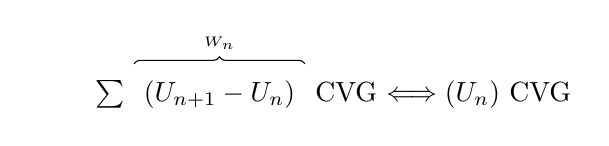
\begin{tikzpicture}[node distance=1mm]
    \node (Let) at (-2, 0) {};

    \node[above right = -0.3cm and 0.5cm of Let] (domain) {$\sum$};
    \node[right = -0.1mm of domain] (codomain) {$(U_{n+1} - U_n)$};
    \node[right = 0.1mm of codomain] (Rcodomain) {CVG $\Longleftrightarrow (U_n)$ CVG};
    \draw [decorate, decoration={brace, raise=2.5pt}] (codomain.north west) -- (codomain.north east) node [ midway,sloped,above = 0.15cm] {\tiny $W_n$};
    
\end{tikzpicture}

\paragraph{Example}
\begin{enumerate}
    \item ⚠ General Example, limit calculation:
     \begin{align*}
        \bf S_n = \sum\limits_{k=0}^{n} W_k = \sum\limits_{k=0}^n \left(U_{k+1} - U_k\right) &= \sum\limits_{k=0}^n U_{k+1} - \sum\limits_{k=0}^n U_k\\
        &= \sum\limits_{k=1}^{n+1} U_k - \sum\limits_{k=0}^n U_k\\
        &= \left(\sum\limits_{k=1}^{n} U_k + U_{n+1}\right) - \left(U_0 + \sum\limits_{k=1}^n U_k\right)\\
        Sn & = \sum\limits_{k=0}^n \left(U_{k+1} - U_k \right) = U_{n+1} - U_0
        \end{align*}
    \item 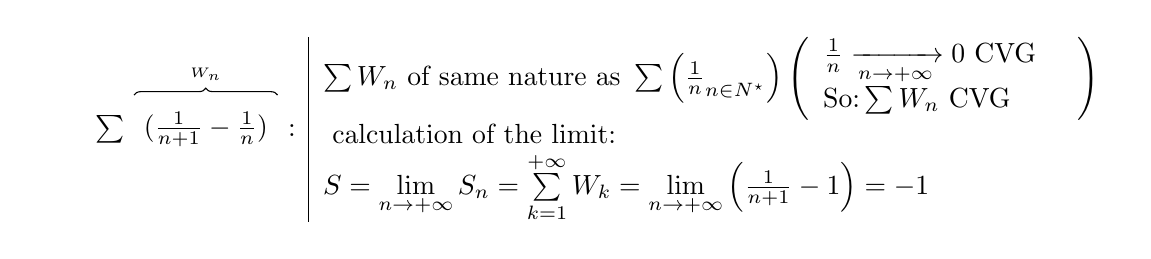
\begin{tikzpicture}[node distance=1mm]
        \node (Let) at (2, 0) {};
    
        \node[right = 0.5cm of Let] (domain) {$\sum$};
        \node[right = -0.1mm of domain] (codomain) {$(\frac{1}{n+1}-\frac{1}{n})$};
        \node[right = 0.1mm of codomain] (Rcodomain) {: $\begin{array}{|l}
        \sum W_n \text{ of same nature as } \sum \left(\frac{1}{n}_{n \in \mathbb{N}^\star}\right) \left( \begin{array}{ll}
            \frac{1}{n} \xrightarrow[n \to +\infty]{} 0 \text{ CVG}&\\
            \text{So:}  \sum W_n \text{ CVG}&
        \end{array} \right)\\
        \text{ calculation of the limit: }\\
        S = \lim\limits_{n \to +\infty} S_n = \sum\limits_{k=1}^{ +\infty} W_k = \lim\limits_{n \to +\infty} \left(\frac{1}{n+1} - 1\right) = -1
        \end{array}$};
    
        \draw [decorate, decoration={brace, raise=2.5pt}] (codomain.north west) -- (codomain.north east) node [ midway,sloped,above = 0.15cm] {\tiny $W_n$};
    \end{tikzpicture}
    
\end{enumerate}
\subsection{Riemann's Rule}
Let $\bf \sum U_n$ a \underline{Positive} numerical series.
If $\bf \exists \alpha > 1 , n^\alpha \times U_n \underset{+\infty}{\sim} 0$ then $\bf \sum U_n$ CVG
\subsubsection{Proof}
$\bf \exists \alpha > 1, n^\alpha \times U_n \xrightarrow[n \to +\infty]{} 0 \implies \frac{U_n}{\frac{1}{n^\alpha}} \xrightarrow[n \to +\infty]{} 0$\\
$\implies \left\{ \begin{array}{r|r}
    U_n = o(\frac{1}{n^\alpha}) &\\
    \text{and } &\\ 
    \alpha > 1 & \left[ \sum \frac{1}{n^\alpha} \text{ CVG (Riemann's series)} \implies \sum U_n \text{ CVG} \right]\\
    \text{and } &\\
    \sum U_n \text{ P.T.S.}& \\
\end{array} \right. $
\subsection{D'Alembert's Rule}
Let $\bf (U_n)$ be a strictly positive sequence such that:
\[ \frac{U_{n+1}}{U_n} \xrightarrow[n \to +\infty]{} \ell \in \mathbb{R}_+\cup \{+\infty\} \]
Then:
$\begin{array}{l}
    \ell < 1 \implies \sum U_n \text{ CVG}\\
    \ell > 1 \implies \sum U_n \text{ DVG}\\
    \ell = 1 \implies \text{ no conclusion}    
\end{array}$
\subsubsection{Example}
$\bf \sum \frac{1}{n!}$ : $\forall n \in \mathbb{N}, \frac{1}{n!} > 0$ (P.T.S.) and $\frac{U_{n+1}}{U_n} = \frac{\frac{1}{(n+1)!}}{\frac{1}{n!}} = \frac{1}{n+1} \xrightarrow[n \to +\infty]{} 0 < 1 \implies \sum \frac{1}{n!}$ CVG\\

\subsection{Cauchy's Rule}
Let $\bf (U_n)$ be a strictly positive sequence such that:
\[ \sqrt[n]{U_n} \xrightarrow[n \to +\infty]{} \ell \in \mathbb{R}_+\cup \{+\infty\} \]
Then:
$\begin{array}{l}
    \ell < 1 \implies \sum U_n \text{ CVG}\\
    \ell > 1 \implies \sum U_n \text{ DVG}\\
    \ell = 1 \implies \text{ no conclusion}
\end{array}$
\subsubsection{Example}
$\bf \sum {(\frac{n}{n+1})^n}^2$: $\forall n \in \mathbb{N}, {(\frac{n}{n+1})^n}^2 > 0$ (P.T.S.), $\sqrt[n]{U_n} = \left({(\frac{n}{n+1})^n}^2\right)^{\frac{1}{n}} = (\frac{n}{n+1})^n = e^{n \ln(1 - \frac{n}{n+1})}$\\[0.2cm]
$\ln(1 - \frac{n}{n+1}) \sim n \times (-\frac{n}{n+1}) \xrightarrow[n \to +\infty]{} -1 < 0 \implies \sqrt[n]{U_n} \xrightarrow[n \to +\infty]{} e^{-1} = \frac{1}{e} < 1 \underset{\text{Cauchy}}{\implies} \sum U_n$ CVG\\
\subsection{Examples}
\begin{enumerate}[label=\protect\circled{\arabic*}]
    \item $\sum (1 + \frac{1}{n})^n$: $1 + \frac{1}{n} \centernot{\xrightarrow[n \to +\infty]{}} 0$ (don't have the necessary condition) $\implies \sum (1 + \frac{1}{n})^n$ DVG\\
    \item $\sum \left((1 + \frac{1}{n})^n - e\right)$: 
    \begin{enumerate}
        \item   \begin{align*}
             \left((1 + \frac{1}{n})^n - e\right) = e^{n \times \ln(1 + \frac{1}{n})} - e &= e^{n \times (\frac{1}{n} - \frac{1}{2n^2} + o(\frac{1}{n^2}))} - e \\
             &= e^{1 - \frac{1}{2n} + o(\frac{1}{n})} - e \\
             &= e \times e^{-\frac{1}{2n} + o(\frac{1}{n})} - e \\ &= e \times (1 - \frac{1}{2n} + o(\frac{1}{n})) - e \\ &= -\frac{e}{2n} + o(\frac{1}{n})
            \end{align*}
            So $\left((1 + \frac{1}{n})^n - e\right) \underset{+\infty}{\sim} -\frac{e}{2n}$ (Can't use P.T.S. property)
        \item $\sum -\frac{e}{2n} < 0$ for $ n \in \mathbb{N}^\star$
        \item $\exists p \in \mathbb{N}^\star, (n \geq p) \implies (\left((1 + \frac{1}{n})^n - e\right) \leq 0)$ (Same sign as $\sum -\frac{e}{2n}$) \\[0.2cm]
        $\implies \sum \left((1 + \frac{1}{n})^n - e\right)$ has the same nature as $\sum -\frac{e}{2n}$ wich is of same nature as $\sum \frac{1}{n}$ DVG
    \end{enumerate}
    \item $\sum n^{2023} \times e^{-n} = \sum \frac{n^{2023}}{e^n}$: $n^{2023} = o(e^n)$ (growth comparison)
    $n^{2025} \times e^{-n} = \frac{\frac{n^{2023}}{e^n}}{\frac{1}{n^2}} \xrightarrow[n \to +\infty]{} 0 \implies U_n = o(\frac{1}{n^2}) \underset{\text{Riemann} (\alpha = 2>1)}{\implies} \sum U_n$ CVG\\
    \item $\sum n! \times e^{-n}$\\
\end{enumerate}
\section{Alternating Series}
\subsection{Definition}
Let $\bf (U_n) \in \mathbb{R}^\mathbb{N}$, we say $\bf (U_n)$ is an alternating sequence thus $\bf \sum U_n$ an alternating series, if there exists $\begin{array}{|l} \text{a positive} \\ \color{green}\text{a negative}\end{array}$ sequence $\bf (a_n)$ such that:
\[\bf \forall n \in \mathbb{N}, \begin{array}{|l} U_{n} = (-1)^n \times a_n \\ \color{green} U_{n} = (-1)^{n+1} \times a_n \end{array}\]
\subsubsection{Example}
$\bf \sum \frac{(-1)^n}{n}$ is an alternating series because $\bf \forall n \in \mathbb{N}, \frac{(-1)^n}{n} = (-1)^n \times \frac{1}{n}$
\subsection{Alternating Series Special Criteria (A.S.S.C.)}
\subsubsection{Theorem}
Let $\bf (U_n)$ an alternating sequence, such that:
\[\bf \left. \begin{array}{l}
    U_n \xrightarrow[n \to +\infty]{} 0\\
    (\left\lvert U_n \right\rvert )_{n \in \mathbb{N}} \text{ is decreasing}
\end{array} \right] \implies \sum U_n \text{ CVG}\]
\subsubsection{Explanation}
An alternating sequence is of the form 
\begin{align*}
    \bf U_n = (-1)^n \times a_n & \qquad \text{ or } & \bf U_n = (-1)^{n+1} \times a_n\\
\bf \left\lvert U_n \right\rvert = \left\lvert (-1)^n \times a_n \right\rvert = \left\lvert a_n \right\rvert & \qquad \text{ or } & \bf \left\lvert U_{n} \right\rvert = \left\lvert (-1)^{n+1} \times a_{n} \right\rvert = \left\lvert a_{n} \right\rvert\\
\text{So }& \bf (\left\lvert U_n \right\rvert )_{n \in \mathbb{N}} = (a_n)_{n \in \mathbb{N}}&\\
\end{align*}
\section{Absolute Convergence}
\subsection{Definition}
Let $\bf (U_n)$ a sequence, we say $\bf \sum U_n$ is absolutely convergent if $\bf \sum \left\lvert U_n \right\rvert$ is convergent.
\subsubsection{Example}
$\bf \sum \frac{(-1)^n}{n^2}$ is absolutely convergent because $\bf \sum \left\lvert \frac{(-1)^n}{n^2} \right\rvert = \sum \frac{1}{n^2}$ is convergent.
\subsection{Proposition}
Let $\bf \sum U_n$ a series, if $\bf \sum U_n$ is absolutely convergent then $\bf \sum U_n$ is convergent.
\[\bf \sum \left\lvert U_n \right\rvert \text{ CVG } \begin{array}{l}  \implies \\ {\color{red}\centernot{\color{black}\Longleftarrow}} \end{array} \bf \sum U_n \text{ CVG.}\]
\subsubsection{Counter Example}
$\bf \sum \frac{(-1)^n}{n}$ is convergent BUT $\bf \sum \left\lvert \frac{(-1)^n}{n} \right\rvert = \sum \frac{1}{n}$ is divergent.
\end{document}